\chapter{Praktični rad} \label{chapter_practical}

\textit{Mirai} je zloćudni program koji napada uređaje interneta stvari 
 s Linux operacijskim sustavom. Ranjive uređaje skuplja u botnet mrežu te 
 koordinira raspodijeljeni napad uskraćivanjem usluga (engl., \textit{Distributed Denial of 
 Service}, skr., \textit{DDoS}). Na ranjive uređaje prenosi program 
 \textit{bot} koji ima ulogu klijenta u \textit{Command And Control} 
 arhitekturi. Bot na zapovijed napadača izvodi DDoS napad, skenira mrežu u
 potrazi za novim žrtvama te ima mogućnost brisanja svoje izvršne datoteke 
 zbog čega ostavlja minimalan trag u sustavu. Uređaje napada pogađajući 
 njihovu IP adresu te pogađajući korisničko ime i lozinku za servise \textit{SSH} i 
 \textit{telnet}. Kombinacije koje isprobava su one koje su najčešće korištene ili one
 koje su postavljene kao zadane na popularnijim uređajima interneta stvari --
 poput najprodavanijih IP kamera i usmjeritelja (engl.,
 \textit{router}). Napad na tvrtku DYN 2016. godine prouzročio je pad većine
 popularnih servisa poput GitHuba, Twittera, Reddita, Netflixa i AirBnBa, a
 napad na tvrtku OVH 2016. godine je generirao promet veličine 1 Tbps 
 \cite{Ling2020}. Procijenjeno je da je najviše zaraženih uređaja u jednom
 trenutku bilo oko 600 000 \cite{Ling2020}.

 Autor je izvorni kôd programa javno objavio što je uzrokovalo pojavu 
 varijanti zloćudnih programa koji danas tvore familiju Mirai zloćudnih programa.
 Varijante napadaju širi spektar uređaja i arhitektura, pa primjerice varijante
 \textit{SORA} i \textit{UNSTABLE} napadaju sustave za pohranu snimki nadzornih
 kamera \cite{sora_unstable}, a \textit{Okiru} napada posebno procesore s ARC
 arhitekturom. 
 % do sada napada i broj zarazenih uređaja
 % navedi neke varijante
 % Napada više arhitektura, traži defaultne lozinke, C&C
 % sad je cijela familija

U ovom radu opisan je postupak generalizacije i klasifikacije zloćudnih 
programa familije \textit{Mirai} korištenjem rudarenja podataka. Opisana je
teorija postupka te je opisana napravljena implementacija, odnosno pronalaženje
zajedničkih svojstava svim programima iz familije.

\section{Definicija problema otkrivanja familije}
Zbog formiranja familije, odnosno skupa zloćudnih programa s istim svojstvima i
nastalim iz istog izvornog koda, postavljen je problem generalizacije familije.

Promatrajući općenita svojstva familije Mirai, postavljena su temeljna
ograničenja rješenja problema:
\begin{enumerate}
    \itemsep0em 
    \item zbog brisanja izvršne datoteke programa, teško je pronaći virus
skeniranjem trajne memorije (tvrdog diska);
    \item familija napada razne arhitekture, ali specifično operacijski sustav
    Linux;
    \item zloćudni program na žrtvu prenosi ili napadač ili druge, već zaražene,
    žrtve;
    \item sve varijante nastale su iz, ili po uzoru na, isti izvorni kod,
    \item varijante mogu biti \textit{packirane};
    \item varijante mogu mijenjati svoj \textit{payload};
    \item u programe je moguće dodavati lažne funkcije i funkcionalnosti.

\end{enumerate}

U ovom radu, problem je sveden na analizu (generaliziranje) izvršnih datoteka 
bota koji se prenose na žrtve u svrhu klasifikacije pojedinog izvršnog koda u 
kojem se pokušava odrediti pripada li neki izvršni kod Mirai familiji ili ne.
Tim pristupom je zaobiđeno prvo ograničenje jer se skenira mreža, a ne trajna
memorija. 

\begin{figure}[htb]
    \centering
    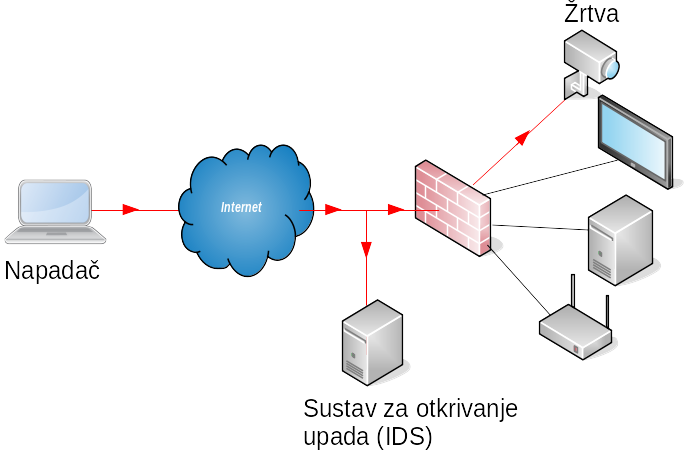
\includegraphics[scale=0.5]{images/IDS_napad.png}
    \caption{Prikaz prijenosa izvršnog koda programa s napadača na žrtvu.
    Crvena linija prikazuje tok podataka.}
    \label{fig:ids_napad}
\end{figure}

Ovakva definicija problema omogućuje implementaciju rješenja u sustav u kojem
se program za klasifikaciju nalazi na sustavima za otkrivanje upada (IDS).
Primjer takvog napada i sustava prikazan je na slici \ref{fig:ids_napad}. IDS 
konstantno prisluškuje dolazeći promet, izdvaja ELF izvršne datoteke i 
zaključuje pripada li datoteka Mirai familiji.

 % imamo razne arhitekture
 % packiranje (enkriptiranje?)
 % "svi na istu foru"
 % obfuskacija koda
 % odgovori na pitanje: gdje se ovo rjesenje moze koristiti?
 %      ne ostaje na hard disku
 %      detekcija prijenosa programa bota


\section{Opis pristupa} %Opis metode?

 % imamo bazu raznih mirai varijanti
 % svaku varijantu simbolicki izvrsimo i zabilježimo sustavske pozive
 % iz tragova sustavskih poziva stvorimo SCDG graf
 % dalje izvuci algoritam

 % pokazi kako s kojim korakom eliminiramo opasnosti navedene gore
 %    stvori primjer za packing
 Pristup korišten u ovom radu izdvaja semantičko ponašanje programa. Semantičko 
 ponašanje opisano je grafovima ovisnosti sustavskih poziva (engl., 
 \textit{System Call Dependency Graph}, skr., \textit{SCDG}), odnosno svaki 
 program predstavljen je sustavskim pozivima koje poziva. Programi su pokrenuti 
 u simuliranom okruženju i tehnikom simboličkom izvršavanja. Simboličko 
 izvršavanje prolazi više mogućih puteva izvršavanja programa, na način da 
 varijablama ne dodjeljuje konkretne vrijednosti, već pri svakom uvjetu 
 razdvaja simulaciju na više mogućih stanja. Nad SCDG grafovima svih izvršnih
 datoteka u bazi, primijenjen je algoritam rudarenja grafova koji kao rezultat 
 daje najčešće podgrafove u ulaznim grafovima -- pretpostavka je da takvi 
 grafovi najbolje opisuju ponašanje familije te takvi podgrafovi postaju
 svojevrstan potpis familije. Koraci izdvajanja potpisa
 prikazani su dijagramom \ref{fig:mining}. U sljedećim potpoglavljima opisan 
 je svaki prethodno navedeni korak.


 \begin{figure}[htb]
    \centering
    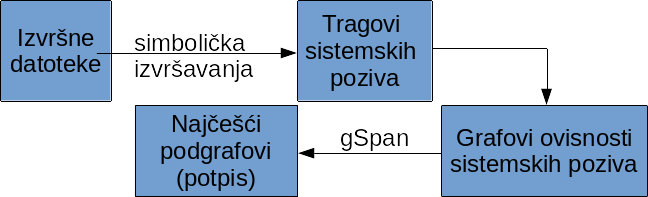
\includegraphics[scale=0.5]{images/mining.png}
    \caption{Dijagram izvlačenja potpisa iz skupa izvršnih datoteka.}
    \label{fig:mining}
\end{figure}

\pagebreak
\subsection{Simboličko izvršavanje i tragovi sustavskih poziva}
Simboličko izvršavanje je metoda statičke analize koda u kojoj se izvođenje
programa simulira, a svaka nepoznata varijabla opisana je simbolima te se naziva
simbolička varijabla. Simbolička varijabla nema konkretnu vrijednost već sadrži
skup ograničenja (uvjeta) koje ispunjava. Svaki novi uvjet nad simboličkom
varijablom razdvaja trenutno stanje simulacije na dva nova stanja -- jedno u
kojem uvjet vrijedi, a drugo u kojem uvjet ne vrijedi. Pojedino stanje
simulacije  sadrži informacije o svim varijablama korištenim u izvođenju. Na 
taj način izvršavanjem se obilaze sve moguće grane izvršavanja.

 Na dijagramu \ref{fig:simbolic_skica} prikazano
je simboličko izvršavanje programa prikazanom u programskom kodu 
\ref{cod:simbolicki_program}. Na dijagramu \ref{fig:simbolic_skica} 
pravokutnicima su prikazana stanja simulacije. Gornji dio pravokutnika sadrži
trenutnu naredbu na kojoj se simulacija nalazi, a donji dio sadrži skupove
uvjeta korištenih simboličkih varijabli. Strelice prikazuju koja stanja
nastaju iz kojeg. Početno stanje je prikazano na vrhu, a završna stanja su ona
iz kojih više nema novih stanja i nalaze se pri dnu. Početno stanje ne sadrži
niti jednu simboličku varijablu -- varijabla \inlinecode{a} postavljena je na
vrijednost 0. Nakon poziva naredbe \inlinecode{scanf} varijabla \inlinecode{a} postaje
simbolička. Zbog uvjeta u programskom kodu na linijama 4-10 varijabla
\inlinecode{a} može poprimiti 3 različita skupa ograničenja te se stanje
razdvaja na tri sljedeća moguća stanja. Skup uvjeta simboličke varijable u 
svakom trenutku mora biti zadovoljiv pa ako je postavljen uvjet simboličke
varijable \inlinecode{a == 3}, uvjet \inlinecode{a < 0} na liniji 13 neće 
biti ispunjen.

Prilikom simboličkog izvršavanja ne pozivaju se stvarni sustavski pozivi, već
se oni simuliraju. Osim simuliranja sustavskih poziva, moguće je simulirati i
funkcije vanjskih programskih knjižnica koje program koristi. Zbog simuliranja
sustavskih poziva, preciznost simulacije (podudarnost simulacije sa stvarnim
izvršavanjem) ovisi o kvaliteti implementacije simulacije.

Trag sustavskih poziva (engl., \textit{system call trace}) čine svi sustavski 
pozivi pozvani u jednoj grani izvođenja programa kod simboličkog 
izvršavanja. sustavski pozivi su poredani slijedno po trenutku poziva te su
navedene vrijednosti parametara i vrijednost koju su vratili (ako postoji). Za
program \ref{cod:simbolicki_program} prikazan je trag \ref{cod:syscall_trace} 
sustavskih poziva za granu izvođenja kad varijabla \inlinecode|a| ima 
vrijednost 4. Svaki sustavski poziv zapisan je u obliku
\inlinecode|ime_poziva(vrijednosti_parametara) = povratna_vrijednost|. Trag je
dobiven programom \inlinecode|strace| \cite{strace_url}, a unesena vrijednost za varijablu
\inlinecode|a| je 4.



% \pagebreak
\begin{lstlisting}[caption={Primjer programa nad kojim je izvršena simboličko pokretanje},label={cod:simbolicki_program}]
int main(void) {
    int a;
    scanf("%d", &a);
    if(a == 3) {
        printf("a == 3");
    } else if (a >= 4) {
        printf("a >= 4");
    } else {
        printf("a != 3 && a < 4");
    }
    printf("\n");

    if(a < 0) {
        printf("a < 0");
    } else {
        printf("a >= 0");
    }
    printf("\n");

    return 0;
}
\end{lstlisting}

\begin{figure}[htb]
    \centering
    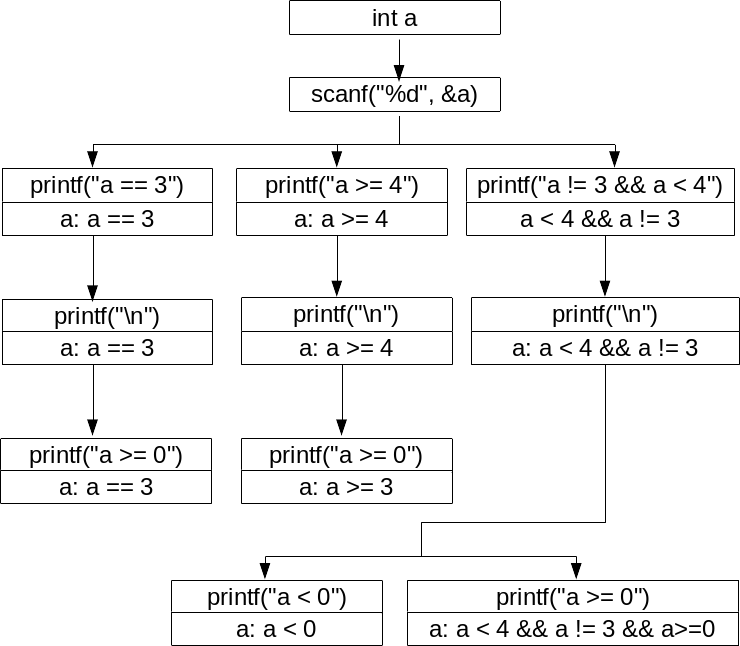
\includegraphics[scale=0.25]{images/simbolic_skica.png}
    \caption{Stanja simboličkog pokretanja za program \ref{cod:simbolicki_program}}
    \label{fig:simbolic_skica}
\end{figure}


\pagebreak
\begin{lstlisting}[caption={Trag sustavskih poziva programa \ref{cod:simbolicki_program} dobiven programom \inlinecode|strace|, uz unos znaka "4" na standardni ulaz},label={cod:syscall_trace}]
execve("./main", ["./main"], 0x7ffc358ee790 /* 57 vars */) = 0
brk(NULL)                               = 0x55ea270a7000
arch_prctl(0x3001 /* ARCH_??? */, 0x7fffbff26b00) = -1 EINVAL (Invalid argument)
access("/etc/ld.so.preload", R_OK)      = -1 ENOENT (No such file or directory)
openat(AT_FDCWD, "/etc/ld.so.cache", O_RDONLY|O_CLOEXEC) = 3
fstat(3, {st_mode=S_IFREG|0644, st_size=126534, ...}) = 0
mmap(NULL, 126534, PROT_READ, MAP_PRIVATE, 3, 0) = 0x7f6624bb4000
close(3)                                = 0
openat(AT_FDCWD, "/lib/x86_64-linux-gnu/libc.so.6", O_RDONLY|O_CLOEXEC) = 3
read(3, "177ELF21130000000030>01000360q200000"..., 832) = 832
pread64(3, "60004000@0000000@0000000@0000000"..., 784, 64) = 784
pread64(3, "4000200005000GNU0200300400030000000", 32, 848) = 32
pread64(3, "4000240003000GNU0\t233222%2742603203133132610204276X>263"..., 68, 880) = 68
fstat(3, {st_mode=S_IFREG|0755, st_size=2029224, ...}) = 0
mmap(NULL, 8192, PROT_READ|PROT_WRITE, MAP_PRIVATE|MAP_ANONYMOUS, -1, 0) = 0x7f6624bb2000
pread64(3, "60004000@0000000@0000000@0000000"..., 784, 64) = 784
pread64(3, "4000200005000GNU0200300400030000000", 32, 848) = 32
pread64(3, "4000240003000GNU0\t233222%2742603203133132610204276X>263"..., 68, 880) = 68
mmap(NULL, 2036952, PROT_READ, MAP_PRIVATE|MAP_DENYWRITE, 3, 0) = 0x7f66249c0000
mprotect(0x7f66249e5000, 1847296, PROT_NONE) = 0
mmap(0x7f66249e5000, 1540096, PROT_READ|PROT_EXEC, MAP_PRIVATE|MAP_FIXED|MAP_DENYWRITE, 3, 0x25000) = 0x7f66249e5000
mmap(0x7f6624b5d000, 303104, PROT_READ, MAP_PRIVATE|MAP_FIXED|MAP_DENYWRITE, 3, 0x19d000) = 0x7f6624b5d000
mmap(0x7f6624ba8000, 24576, PROT_READ|PROT_WRITE, MAP_PRIVATE|MAP_FIXED|MAP_DENYWRITE, 3, 0x1e7000) = 0x7f6624ba8000
mmap(0x7f6624bae000, 13528, PROT_READ|PROT_WRITE, MAP_PRIVATE|MAP_FIXED|MAP_ANONYMOUS, -1, 0) = 0x7f6624bae000
close(3)                                = 0
arch_prctl(ARCH_SET_FS, 0x7f6624bb3540) = 0
mprotect(0x7f6624ba8000, 12288, PROT_READ) = 0
mprotect(0x55ea26f21000, 4096, PROT_READ) = 0
mprotect(0x7f6624c00000, 4096, PROT_READ) = 0
munmap(0x7f6624bb4000, 126534)          = 0
fstat(0, {st_mode=S_IFCHR|0620, st_rdev=makedev(0x88, 0x1), ...}) = 0
brk(NULL)                               = 0x55ea270a7000
brk(0x55ea270c8000)                     = 0x55ea270c8000
read(0, "2\n", 1024)                    = 2
fstat(1, {st_mode=S_IFCHR|0620, st_rdev=makedev(0x88, 0x1), ...}) = 0
write(1, "a != 3 && a < 4\n", 16)       = 16
write(1, "a >= 0\n", 7)                 = 7
lseek(0, -1, SEEK_CUR)                  = -1 ESPIPE (Illegal seek)
exit_group(0)                           = ?
\end{lstlisting}

\pagebreak

\textit{Packeri} su programski alati koji služe za obfuskaciju binarnog koda
izvršne datoteke na način da njihove podatke sažmu ili enkriptiraju. Služe za
otežavanje statičke analize zloćudnog programa. Korištenjem simboličkog 
izvršavanja zaobilazi se problem otkrivanja \textit{packiranog} zloćudnog 
programa jer se simboličkim izvršavanjem program u početku sam otpakira ili
dekriptira.

% TODO packiraj if/else i vidi da je isti.

\subsection{Usmjereni graf ovisnosti sustavskih poziva} %Mozda "Izvlačenje semantičkog ponašanja"

Trag sustavskih poziva opisuje kako program komunicira s operacijskim sustavom,
no ne prikazuje direktno veze između pojedinih pozvanih sustavskih poziva. Zbog
toga se definira usmjereni graf ovisnosti sustavskih poziva (\textit{engl}., 
System Call Dependency Graph, skr., \textit{SCDG}). Čvorovi grafa 
predstavaljaju pozvane sustavske pozive, a lukovi (usmjereni bridovi) opisuju
tok informacija. Smjer luka određen je redoslijedom izvršavanja sustavskih 
poziva -- luk ima smjer od starijeg prema novijem, a dva čvora su spojena ako
dijele istu vrijednost argumenata ili ako se povratna vrijednost starijeg poziva
nalazi kao argument u nekom novijem.

Prikaz stvaranja SCDG grafa prikazan je za program \ref{cod:scdg_prog_prim}.
Program pročita najviše 512 znakova iz datoteke \inlinecode|dat1| i zapiše ih u
datoteku \inlinecode|dat2|. Za dani primjer generiran je trag sustavskih
poziva \ref{cod:trag_scdg_prog_prim}, ali su u tragu navedeni samo sustavski
pozivi bitnu za samu srž aplikacije -- kopiranje znakova iz jedne datoteke u
drugu. Zbog ograničenja alata za crtanje grafova slika ne sadržava višestruke
bridove ni čvorove s istim oznakama. Ako su dva čvora povezana s
više bridova, tada je prikazan samo jedan brid, a oznake stvarnih bridova su
spojene u jednu koristeći zarez -- primjer je brid s oznakom
\inlinecode|1->3,3->3| između čvorova \inlinecode|read_3| i 
\inlinecode|read_4|. Oznakama čvorova nadodan je i broj koji označava poredak
pozivanja sustavskog poziva, a primjeri su čvorovi \inlinecode|read_3| i 
\inlinecode|read_4|.

\newpage

% TODO? reci da od jednog traga dobijes nepovezan graf.

\begin{lstlisting}[caption={Tekst programa za programski jezik C koji prvih 512 okteta jedne datoteke upisuje u drugu},label={cod:scdg_prog_prim}]
int main(void) {
    const char *pathname = "dat1";
    const char *pathname2 = "dat2";

    char buf[512];

    FILE * f = fopen(pathname, "r");
    FILE * f2 = fopen(pathname2,  "w");
    int n = fread(buf, 1, 512, f);
    fwrite(buf, 1, n, f2);
    fclose(f);
    fclose(f2);
}
\end{lstlisting}

\begin{lstlisting}[caption={Dio traga sustavskih poziva dobiven programom \inlinecode|strace|},label={cod:trag_scdg_prog_prim}]
openat(AT_FDCWD, "file.txt", O_RDONLY)  = 3
openat(AT_FDCWD, "file2.txt", O_WRONLY|O_CREAT|O_TRUNC, 0666) = 4
fstat(3, {st_mode=S_IFREG|0664, st_size=16, ...}) = 0
read(3, "Ovo je primjer.\n", 4096)      = 16
read(3, "", 4096)                       = 0
fstat(4, {st_mode=S_IFREG|0664, st_size=0, ...}) = 0
close(3)                                = 0
write(4, "Ovo je primjer.\n", 16)       = 16
close(4)                                = 0
\end{lstlisting}

\begin{figure}[htb]
    \centering
    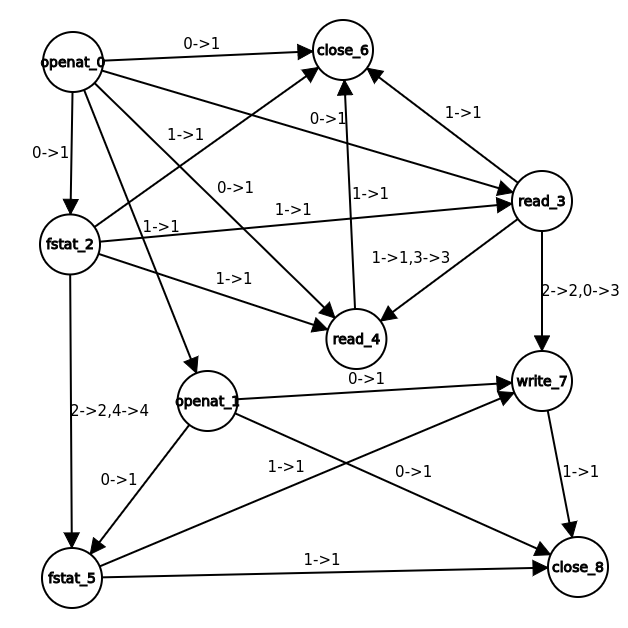
\includegraphics[scale=0.5]{images/scdg_graf.png}
    \caption{Graf ovisnosti sustavskih poziva za trag \ref{cod:scdg_prog_prim}}
    \label{fig:scdg_graf_1}
\end{figure}

\subsubsection{Prednosti SCDG grafova}

Izmjenu originalnog zloćudnog programa moguće je ostvariti ubacivanjem lažnih
ili redundantnih funkcija u programski kod te izmjenom redoslijeda nepovezanih
funkcionalnosti programa \cite{mirai_main}. Dodavanjem redundantnih funkcija u
program, SCDG graf dobiva nove čvorove i bridove, ali se ne gube čvorovi i
bridovi izvornog grafa. Izmjena redoslijeda pojedinih sustavskih poziva može
izmijeniti SCDG graf, ali samo na način da artefaktni bridovi (iz poglavlja
2.2.3) promijene smjer, tako da su bridovi koji zapravo opisuju ponašanje
netaknuti.
% TODO MOZDA NIJE TOCNO

\subsubsection{Nedostaci SCDG grafova}


Prilikom izgradnje SCDG grafa korištenjem prethodno definiranih pravila,
vidljivi su poneki artefakti. Primjer je veza između čvorova
\inlinecode|openat_0| i \inlinecode|openat_1| koja nastaje zbog toga što dijele
isti parametar prvi parametar. Prvi parametar je zapravo konstanta 
\inlinecode|AT_FDCWD| koja označava da je predana putanja relativna i često ju
koristi svaki \inlinecode|openat| sustavski poziv. Bridovi koji nastaju zbog
takvih konstanti nemaju semantičku vrijednost promatrajući izvođenje programa,
ali unose šum koji usporava rudarenje takvih grafova (zbog povećanog broja bridova).

% te je smjer luka određen redoslijedom
% izvršavanja sustavskih poziva -- luk ima smjer od ranijeg prema kasnijem % TODO
% sustavskom pozivu. Dva sustavska poziva su povezana ako 

%Svaki zapis u tragu sustavskih poziva
%predstavlja jedan čvor u SCDG grafu, a čvoru se dodijeljuje oznaka (engl.,
%\textit{label}) koja odgovara imenu sustavskog poziva. Bridovi su usmjereni, a
%povezuju dva čvora čiji sustavski pozivi imaju istu vrijednost nekog parametra
%i/ili 

\subsection{Izvlačenje znanja i klasifikacija}

Jedan od načina izvlačenja znanja iz skupa grafova je rudarenje učestalih
podgrafova (engl., \textit{Frequent Subgraph Mining}, skr., \textit{FSM}).
U kontekstu SCDG grafova, gdje pojedini graf predstavlja ponašanje programa,
učestali podgrafovi predstavljaju učestala ponašanja skupine programa. Algoritmi
za FSM razlikuju se po tome daju li potpuno rješenje (poput algoritama gSpan i 
AGM) ili aproksimaciju (algoritam SLEUTH). Algoritmi kao hiperparametre primaju
broj učestalih podgrafova koji trebaju vratiti te broj koji govori u koliko se
grafova mora nalaziti podgraf da bi se smatrao učestalim. Rezultat FSMa nad SCDG
grafovima je svojevrstan potpis koji se kasnije koristi u klasifikaciji.

U ovom radu je korišten gSpan, odnosno njegova implementacija zvana quickSpan.
Kod izvlačenja potpisa algoritmu \textit{gSpan} predan je hiperparametar
\textit{support} te su rezultantni podgrafovi poredani po veličini te se kao
krajnji rezultat smatra \textit{n} najvećih. Pseudokod je prikazan u
\ref{psd:izvuci_potpis}. Kod klasifikacije, provjerava se sadrži li graf
podgrafove iz potpisa. Prolazeći kroz svaki podgraf iz potpisa, algoritmom
\textit{gSpan} izdvoje se svi podgrafovi koje sadrži i podgraf iz potpisa i graf
kojeg klasificiramo. Nakon toga ispituje se sličnost takvih podgrafova i
podgrafa potpisa i ako su slični, tada je graf klasificiran kao da pripada
traženom razredu. Mjera sličnosti grafova definirana je kao omjer broja bridova
grafova. Jednadžba je prikazana slikom \ref{eqn:mjera_slicnosti}. \\

\SetKwInput{Gin}{G}
\SetKwInput{Support}{support}
\SetKwInput{n}{n}
\SetKwInput{threshold}{threshold}

\SetKwData{Gin}{G}
\SetKwData{g}{g}
\SetKwData{n}{n}
\SetKwData{Support}{support}
\SetKwData{Sign}{sign} 
\SetKwData{CSG}{CSG}
\SetKwData{MaxCSG}{maxCSG}
\SetKwData{gsig}{g\_1}
\SetKwData{gsigsig}{g\_2}
\SetKwData{subsubG}{subsubG}

\SetKwFunction{gSpan}{gSpan}
\SetKwFunction{GraphSim}{slicnost\_grafova}
\SetKwFunction{sortiraj}{sortiraj}

\begin{algorithm}[H]
    \caption{Izvlačenje potpisa iz skupa grafova koristeći gSpan algoritam
    \label{psd:izvuci_potpis}
    }

    \KwIn{\Gin: skup SCDG grafova}
    \KwIn{\Support: hiperparametar gSpan algoritma}
    \KwOut{\Sign: skup podgrafova koji čine potpis}

    \Sign$\leftarrow \{\emptyset\}$ \;
    \CSG$\leftarrow$ \gSpan{\Gin, \Support} \;
    \MaxCSG$\leftarrow$ \sortiraj{\CSG, \n} \tcp*{Dohvati n najvećih učestalih 
    podgrafova}

    \lForEach{\g$ \in$ \MaxCSG}{\Sign$ \leftarrow$ \Sign$ \cup$ \{\g\} }
\end{algorithm}



\begin{algorithm}[H]
    \caption{Klasifikacija SCDG grafa
    \label{psd:klasifikacija}
    }

    \KwIn{\Sign: skup podgrafova koji čine potpis}
    \KwIn{\Support: hiperparametar gSpan algoritma}
    \KwIn{\threshold: prag sličnosti dva grafa}
    \KwOut{Booleova vrijednost spada li graf \g unutar klase ili ne}

    \ForEach{\gsig$ \in$ \Sign}{
        \tcp*[h]{Support hiperparametar je 1} \\
        \subsubG$ \leftarrow$ \gSpan{$\{$\g$, \gsig$$\}$, $1$} \; 
        \ForEach{\gsigsig$ \in$ \subsubG}{
            \If{\GraphSim{\gsigsig$, \gsig$} > \threshold }{\Return{True}}
        }
    }

    \Return{False}

\end{algorithm}

\begin{figure}[htb]
    \centering
    \[M(G_1, G_2) = |E(G_1)|/|E(G_2)| \]
    \caption{Mjera sličnosti grafova koja uzima u obzir omjer broja bridova}
    \label{eqn:mjera_slicnosti}
\end{figure}

% Sto radi
% kako ga i gdje korsitim
% tko ga je napravio i kada
% slozenost

\section{Programsko ostvarenje}



% TODO reci da sam dobio preko honeypota one viruse
U ovom potpoglavlju opisani su implementacijski detalji, korišteni alati i
načini pokretanja napravljenog programa.
%reci da ciljam na armove arhitekture (ima ih vise, navedi koje)

% TODO ? dodati na pocetku "Opis skupa podataka" i info da je koristen dev angr
\subsection{Radni okvir Angr}
Okvir angr je alat za analizu izvršnih datoteka, a napisan je za programski 
jezik Python. Pruža mogućnost simboličkog izvršavanja programa, ali i automatizirano 
otkrivanje sigurnosnih ranjivosti te nudi alate za analizu ponašanja programa,
poput grafa ovisnosti podataka (engl., \textit{Data Dependency Graph}) i grafa
kontrole toka (engl., \textit{Control-Flow Graph}). Sposoban je analizirati
programe za razne procesorske arhitekture (ARM, x86, x64) te razne formate
izvršnih datoteka (ELF i PE/EXE).


Prije početka simulacije, potrebno je učitati izvršnu datoteku i pružiti
Angru sve potrebne vanjske knjižnice, a procesorsku arhitekturu, format
izvršne datoteke i procesorsku arhitekturu alat odredi sam. Simulacija se
provodi koračanjem kroz blokove izvršnog programa, odnosno stanja simulacije. Blok
je dio učitanog izvršnog programa koji sadrži ili predefinirani najveći broj 
instrukcija ili završava uvjetovanom instrukcijom ili instrukcijom skoka.
Stanje simulacije sadrži blok koda te sadržaj registara i memorije, a njezinim
izvršavanjem dobivaju se sljedeća stanja, odnosno sljedbenici. Simulacija
započinje sadržavajući samo jedno početno stanje kojoj blok počinje s
instrukcijama na početku programa. Angr sprema nekoliko različitih
listi stanja, poput listi aktivnih stanja, mrtvih stanja i uspješnih stanja.
Aktivna stanja su ona koja će se izvesti u sljedećem koraku simulacije, a nakon
koraka simulacije sljedbenici tih stanja postaju aktivna stanja. Mrtva stanja su
ona čijim se izvođenjem dogodila greška, a kod uspješnih stanja je izvođenje
simulacije uspješno završeno. Dio programskog koda \ref{cod:angr_sim} prikazuje korištenje
navedenih mehanizama i pokretanje simulacije u Angru.

U ovom radu korišteni su Angrovi mehanizmi prijelomnih točaka (engl.,
\textit{breakpoint}) i dodataka (engl., \textit{plugin}). Korištenjem prijelomne
točke moguće je izvršiti korisnički definiranu funkciju u trenutku kad se dogodi
neki događaj, poput pozivanja sustavskog poziva, zapisivanja i čitanja iz
memorije, ili poziva do tad neviđene instrukcije. U dodacima se spremaju dodatne
informacije vezane uz stanje, a korisnik određuje što se događa u trenutku kad
pojedino stanje nastaje. U ovom radu navedeni mehanizmi iskorišteni su za
pamćenje tragova sustavskih poziva.

\begin{lstlisting}[caption={Dio koda zaslužan za simboličku analizu u angru i učitavanje potrebnih dodataka i vanjskih knjižnica},label={cod:angr_sim}]
    so_dirs = [x[0] for x in os.walk('./arm_libs/armel')]

    proj = angr.Project(os.path.join(BIN_DIR, FILE_NAME),
                        load_options={
                            'auto_load_libs': True, 'except_missing_libs': True, "use_system_libs": False,
                            'ld_path': so_dirs
                        },
                        use_sim_procedures=False)

    start_state = proj.factory.entry_state()

    root_nodes = list()
    start_state.register_plugin('syscall_tree', SyscallTreePlugin())
    start_state.inspect.b('syscall', when=angr.BP_AFTER, action=syscall_tree_action_builder(root_nodes))

    simgr = proj.factory.simgr(start_state)

    print("Exploring binary...")
    simgr.explore(n=400)
    print("Exploring binary finished.")

\end{lstlisting}

\subsection{Ekstrakcija SCDG grafova koristeći okvir Angr}

\subsubsection{Dodavanje prevedenih sustavskih knjižnica}
U ovom radu ciljana arhitektura je ARM, odnosno njegove inačice ARMLE i ARMHF, a
ciljani operacijski sustav je Linux. Svaki dinamički preveden koristi standardne
knjižnice (poput \textit{stdlib.c}) za ispravan rad pa tako i Angru treba
putanja standardnih knjižnica prevedenih za ciljani operacijski sustavi ciljanu
arhitekturu. ARMHF preuzet je iz operacijskog sustava RaspbianOS za arhitekturu
ARM \cite{raspbian_arm}. ARMEL je preuzet iz operacijskog sustava Debian
kompajliranog za ARMEL arhitekturu \cite{armel}. 

\subsubsection{Implementacija nedostajućih sustavskih poziva}
Pokušajem pokretanja analize nad skupom podataka utvrđeno je da postoje
sustavski pozivi koji nisu implementirani. Primjeri takvih sustavskih poziva su
\inlinecode{access}, \inlinecode{connect}, \inlinecode{getsockname}, 
\inlinecode{ioctl}, \inlinecode{readlink}, \inlinecode{rt_sigprocmask},
\inlinecode{set_robust_list} i \inlinecode{set_thread_area}. U nastavku je
prikazana implementacija sustavskog poziva \inlinecode{readlink}. 

sustavski poziv \inlinecode{readlink} učitava vrijednost simboličkog linka 
\cite{readlink_doc}. Funkcija kao parametar prima simbolički link kao niz
znakova, spremnik u koji zapisuje rezultat kao niz znakova i veličinu tog
spremnika. Kao rezultat vraća broj zapisanih znakova u spremniku. Deklaracija
 funkcije prikazana je kodom \ref{cod:readlink_decl}. Ako je kao simbolički 
 link predana vrijednost \inlinecode|/proc/self/exe|,
onda se u spremnik zapisuje puna putanja do izvršne datoteke pokrenutog 
programa. Programi u promatranom skupu podataka pozivaju funkciju isključivo
s tom vrijednošću simboličkog linka te zbog toga implementacija funkcije nije
potpuna, već sadrži samo korišten slučaj. Okolina u kojoj Angr simbolički 
izvršava program je simulirana, no u ovoj implementaciji vraćena je puna 
putanja do simbolički izvršavane izvršne datoteke. Pri definiranju novog
sustavskog poziva u Angru potrebno je stvoriti razred koji nasljeđuje
\inlinecode{SimProcedure} i implementirati metodu \inlinecode{run} koja se
poziva pri pozivanju sustavskog poziva. Klasa je spremljena u datoteku
\inlinecode{procedures/linux_kernel/readlink.py}. 
Nakon toga sustavski poziv je unešen u sustav, no unos nije opisan jer je
postupak predugačak i, trenutno, nije službeno dokumentiran.

\begin{lstlisting}[caption={Deklaracija readlink funkcije},label={cod:readlink_decl}]
    ssize_t readlink(const char *pathname, char *buf, size_t bufsiz);
\end{lstlisting}

\begin{lstlisting}[caption={Implementacija readlink sustavskog poziva za angr},label={cod:readlink_impl}]
class readlink(SimProcedure):
    def run(self, pathname, buf, bufsiz):
        elf_path = (os.getcwd() + "/" + self.state.project.filename).encode('utf-8')
        buffsize_int = self.state.solver.eval(bufsiz)
        elf_path_bvv = claripy.BVV(value=elf_path, size=len(elf_path) * 8)
        store_size = min(buffsize_int, len(elf_path))
        self.state.memory.store(addr=buf, data=elf_path_bvv, size=store_size)
        l.debug('readlink: {} : {} : {} | {}'.format(pathname, buf, buffsize_int, buffsize_int))
        return len(elf_path)
\end{lstlisting}


\subsubsection{Implementacija nedostajućih instrukcija}
Interno, Angr simboličku analizu izvodi nad međukodom kojeg dobije alatom Vex,
kojeg koristi i popularan alat za analizu programa Valgrind. Prilikom pokušaja
simboličke analize nad nekim izvršnim datotekama, uočeno je da trenutna verzija
Vexa koju koristi Angr nema implementiranu instrukciju \inlinecode|rdsspq|.
Instrukcija je dodana u okviru Intelovog sklopovskog proširenja za osiguravanje
kontrole toka (engl., \textit{Control-flow Enforcement Technology}, skr. CET), 
a onemogućuje promjenu adrese povratka iz funkcije koristeći sklopovsku 
podršku. Promjena adrese je onemogućena jer se povratne adrese čuvaju na
rezervnom, tzv., stogu u sjeni (engl., \textit{Shadow stack}) kojem nije moguće 
pristupiti. Prilikom povratka iz funkcije učitava se povratna adresa te ako
učitana povratna adresa ne odgovara onoj sa stoga u sjeni, događa se iznimka koja
signalizira grešku. 

U ovom radu sve naredbe za manipulaciju stoga u sjeni su implementirane kao
prazna instrukcija (eng., \textit{No operation Code}, skr., \textit{NOP}). 
Promjene su napravljene u izvornom kodu alata Vex.


\subsubsection{Stvaranje tragova sustavskih poziva}
Stvaranje tragova sustavskih poziva nije nativno podržano u Angru, već je
izvedeno pomoću proširenja stanja i prijelomnih točaka. Pomoću prijelomnih
točaka moguće je izvršiti neku funkciju u trenutku kada se dogodi događaj u
simulaciji izvođenja programa -- poput ulaska i izlaska iz sustavskog poziva,
čitanja ili zapisivanja u određeni segment memorije, čitanja ili zapisivanja u
određeni registar ili poziv procesorske naredbe. Pomoću proširenja stanja Angr
omogućuje zapisivanje dodatnih informacija u pojedino stanje. Informacije se
prenose (odnosno kopiraju) s izvornog stanja na stanja koja iza njega slijede,
te ih je moguće dinamički mijenjati.

Kod stvaranja tragova sustavskih poziva u svako stanje simulacije upisan je 
zadnji, do tog trenutka pozvani, sustavski poziv i svi njegovi sljedbenici, a 
prekidne točke postavljene su na poziv sustavskog poziva te u zadano 
stanje upisuju informacije o pozvanom sustavskom pozivu te se nadodaje u listu
sljedbenika svog prethodnika. Na taj način je niz tragova sustavskih
poziva zapisan kao skup stabala. Primjer jednog takvog stabla prikazan je slikom
\ref{fig:systrace_tree}. Zbog ograničenja programa za crtanje grafa, uz ime
sustavskog poziva, oznaci čvora nadodan je i redni broj otkrivanja sustavskog
poziva prilikom simulacije.


\begin{figure}[htb]
    \centering
    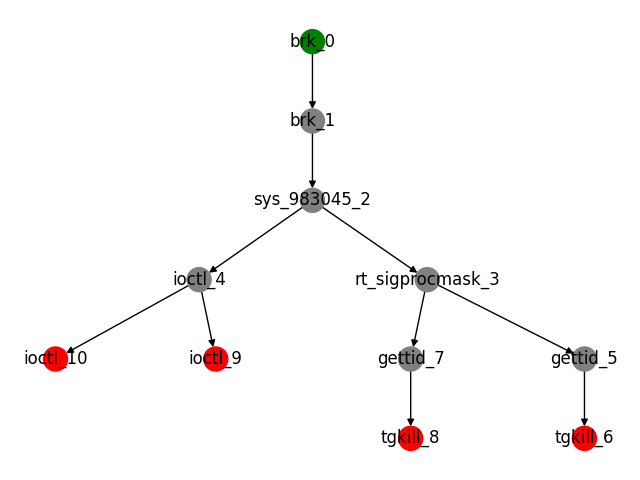
\includegraphics[scale=0.75]{images/systrace_graph.png}
    \caption{Prikaz grafa sustavskih tragova}
    \label{fig:systrace_tree}
\end{figure}



\subsubsection{Stvaranje SCDG grafova iz tragova sustavskih poziva}

Tragovi sustavskih poziva mogu se zamisliti kao usmjerena stabla u kojima su
čvorovi pozvani sustavski pozivi, a bridovi opisuju kronologiju pozivanja
sustavskih poziva -- brid je usmjeren od prethodnika prema sljedbeniku. U ovom
radu, SCDG graf dobiven je obilaženjem tragova sustavskih poziva u dubinu
(engl., \textit{Depth-first Search}, skr., \textit{DFS}) te pamćenjem
vrijednosti koje sustavski pozivi primaju ili vraćaju do trenutno promatranog
čvora. Programski kod \ref{cod:trace_u_scdg} prikazuje funkciju koja prima
korijen stabla i, do tog trenutka, poznate čvorove čiji sustavski pozivi primaju
ili vraćaju određene vrijednosti. Parametar funkcije \inlinecode|parametri| je
rječnik koji mapira vrijednost u listu čvorova sustavskih poziva koji ga
primaju, dok je parametar \inlinecode|povratne_vrijednosti| također rječnik 
koji mapira vrijednost u listu čvorova sustavskih poziva koji ju vraćaju.
Prvi dio funkcije (linije 3 - 15) upisuju trenutni čvor (zapisan u varijabli
\inlinecode|cvor|) u prethodno navedene rječnike u sve liste povezane s
vrijednostima njegovih argumenata koje je primio i vratio. Drugi dio funkcije
(linije 17 i 18) izvode korak rekurzije pozivajući funkciju nad svim
nasljednicima čvora. Treći dio funkcije (linije 20 do 24) brišu informacije
nadodane u drugom koraku. Zadnji dio funkcije (linije 26 do 33) zapisuje 
bridove grafa na način da trenutni čvor povezuje s prethodnicima kod kojih
povratna vrijednost ili vrijednost argumenata njihovih sustavskih poziva postoji
u argumentima sustavskog poziva trenutnog čvora. Smjer brida je od prethodnika
prema sljedbeniku, a oznaka brida je uređeni par dva prirodna broja koji
odgovaraju poziciji na kojoj se određena vrijednost nalazi u argumentima
prethodnog i sljedećeg poziva, uz iznimku da je indeks povratne vrijednosti 
prethodnika označena s nulom, odnosno pozicije argumenata broje se od jedinice. 
\\


\begin{lstlisting}[caption={Rekurzivna funkcija za stvaranje SCDG grafa iz čvora sustavskog traga},label={cod:trace_u_scdg}]
fun stvori_scdg_iz_cvora(cvor, parametri, povratne_vrijednosti):
  
    # Nadodaj sebe u rjecnike "parametri" i "povratna_vrijednost"
    #  da se nasljednici mogu povezati s tobom
    for argument in cvor.sustavski_poziv.argumenti:
      if argument not in parametri:
        parametri[argument] = lista()
      parametri[argument].dodaj(cvor.id)
    
    povratna_vrijednost_poziva = cvor.sustavski_poziv.povratna_vrijednost
    
    if povratna_vrijednost_poziva:
     if povratna_vrijednost_poziva not in povratne_vrijednosti:
       povratne_vrijednosti[povratna_vrijednost_poziva].append(cvor.id)
     
    # Korak rekurzije
    for nasljednik in cvor.nasljednici:
      stvori_scdg_iz_cvora(nasljednik)
    
    # Izbrisi se iz rjecnika "parametri" i "povratna_vrijednost"
    for argument in cvor.sustavski_poziv.argumenti:
      parametri[argument].pop()
    
    povratne_vrijednosti[povratna_vrijednost_poziva].pop()
    
    # Provjeri s kim se trebas povezati od prethodnika
    for argument in cvor.sustavski_poziv.argumenti:
      if argument in parametri:
         for prethodnik in parametri[argument]:
           dodaj_brid(prethodnik, cvor)
      if argument in povratne_vrijednosti:
      for prethodnik in povratne_vrijednosti[argument]:
           dodaj_brid(prethodnik, cvor) 
\end{lstlisting}


\subsection{Treniranje i klasifikacija algoritmom quickSpan}
U ovom radu korištena je quickSpan implementacija gSpan algoritma. 
Implementacija je otvorenog koda te, za razliku od originalne implementacije, 
omogućuje višedretveno izvođenje te je memorijski manje zahtjevna i brža
\cite{quickspan}. Programsko rješenje ima niz opcija pokretanja programa, no u
ovom radu korišteni su sljedeći parametri:
\begin{itemize}
    \item \inlinecode|support| -- \textit{support} hiperparametar gSpan algoritma, 
    \item \inlinecode|input_file| -- putanja do tekstualne datoteke koja sadrži
    ulazne grafove,
    \item \inlinecode|output_file| -- putanja do tekstualne datoteke u koju će
    program upisati rezultat,
    \item \inlinecode|threads| -- broj dretvi koje program treba koristiti,
    \item \inlinecode|directed_graph| -- zastavica koja određuje je li graf usmjeren,
    \item \inlinecode|pattern| -- zastavica koja određuje treba li zapisati rezultat,
    \item \inlinecode|biggest_subgraphs| -- broj koji određuje koliko će prvih
    najvećih podgrafova biti zapisano kao rezultat.
\end{itemize}

Datoteka koja sadrži ulazne grafove mora biti kodirana u UTF-8 formatu, a graf
zapisan na način da se u prvoj liniji navede jedinstveni broj grafa, a nakon
njega definiraju svi njegovi čvorovi i bridovi, zajedno s njihovim oznakama. 
Početak grafa definira se linijom oblika \inlinecode|t # id_grafa|, čvor linijom
\inlinecode|v id_cvora oznaka_cvora|, a brid 
\inlinecode|e id_izlaznog_cvora id_ulaznog_cvora oznaka_brida|. Oznake vrhova i
bridova u quickSpan implementaciji moraju biti pozitivni cijeli brojevi, ali su
bridovi u SCDG grafu označeni s uređenim parom. Zbog toga su bridovi
preimenovani na način da je uređeni par \inlinecode|(x, y)| postaje
\inlinecode|2^x 2^y|. Primjer ulazne datoteke \ref{cod:quickspan_graph} sadrži jedan graf 
prikazan na slici \ref{fig:quickSpan_graph}. Datoteka s rješenjem također je kodirana u UTF-8 formatu
te koristi isti oblik za početak grafa, čvorove i bridove, ali je nadodana i 
informacija o tome koliko i koji grafovi sadrže promatrani podgraf. 



\begin{figure}[htb]
    \centering
    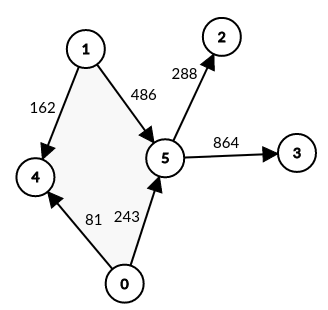
\includegraphics[scale=0.75]{images/quickspan_graph.png}
    \caption{Prikaz grafa za datoteku \ref{cod:quickspan_graph}}
    \label{fig:quickSpan_graph}
\end{figure}

\newpage

\begin{lstlisting}[caption={Primjer ulazne datoteke koja predstavlja graf},label={cod:quickspan_graph}]
t # 0
v 0 0
v 1 4
v 2 1
v 3 5
v 4 2
v 5 3
e 0 1 81
e 2 1 162
e 2 3 486
e 0 3 243
e 3 4 288
e 3 5 864
\end{lstlisting}

Program za pokretanje modela pokreće se naredbom \ref{cod:train_py}, a kao
argumente pri pokretanju prima sljedeće:
\begin{itemize}
    \item \inlinecode|malwares| - putanja do direktorija u kojem se nalaze zloćudni
    programi,
    \item \inlinecode|result| - putanja do datoteke u kojoj se zapisuju rezultati
\end{itemize}

\begin{lstlisting}[caption={Pokretanje treniranja},label={cod:train_py}]
    $ ./train.py --malwares ./data --result ./result
\end{lstlisting}

Program za klasifikaciju izvršne datoteke pokreće se naredbom 
\ref{cod:class_py}, na kraju izvršavanja korisniku ispisuje pripada li izvršna
datoteka familiji, a kao argumente pri pokretanju prima:
\begin{itemize}
    \item \inlinecode|binary| - putanja do datoteke koju se ispituje,
    \item \inlinecode|signature| - putanja do datoteke u kojoj se nalazi
    rezultat treniranja, odnosno potpis familije.
\end{itemize}

\begin{lstlisting}[caption={Pokretanje klasifikacije},label={cod:class_py}]
    $ ./classify.py --binary ./example --signature ./result
\end{lstlisting}

\newpage

\section{Rezultati}
Istraživanje najboljih hiperparametara je preskočeno zbog prevelike složenosti
izvođenja algoritma. Hiperparametar \inlinecode|support| postavljen je na
0.5, a \inlinecode|threshold| sličnosti na 0.46, po najbolje dobivenim
rezultatima iz originalnog rada \cite{mirai_main}. Skup podataka sadržava 407,
po njihovom MD5 sažetku različita, zloćudna programa iz familije Mirai,
prikupljenih u lipnju 2017. godine. Programi
su namijenjeni za arhitekture ARM EABI 4 (196 primjerka), PowerPC ili cisco 4500
(3 primjerka), Intel 8036 (2 primjerka), MIPS (1 primjerak), x86 (1 primjerak),
te nepoznate ARM arhitekture. Arhitekture izvršnih datoteka određene su linux
naredbom \inlinecode|file|. Izvlačenje SCDG grafa Angrom uspješno je za samo 131
zloćudnu izvršnu datoteku. Po uzoru na izvorni rad, skup dobroćudnih datoteka
sastoji se od 131 nasumično odabrane izvršne datoteke iz \inlinecode|/usr/bin|
direktorija za operacijski sustav Ubuntu 20.04 i x86\_64 arhitekturu. Za sve
odabrane izvršne datoteke uspješno je izvučen SCDG graf. 

Pri generiranju potpisa korišteno je 105 (80\%) nasumično odabranih zloćudnih
programa. Pri evaluaciji korišteno je 105 nasumično odabranih zloćudnih
programa i 105 nasumično odabranih dobroćudnih programa. U eksperimentu dobivena
su 3 lažno pozitivna rezultata te 1 lažno negativan. Preciznost je 97.20\%,
odziv je 99.05\%. \inlinecode|F0.5| (koja naglasak stavlja na preciznost, a ne
na odziv) mjera je 0.9756.


\section{Manjkavosti i moguća poboljšanja}

Smatram da su brojne manjkavosti i imam više ideja kako poboljšati ovu metodu. Slobodno se javite na mail, linkedin ili bilo koji 3. servis na kojem me pronađete.

Hrvoje Spajić